\subsection{Baselines}
\label{sec:baselines}

\boldparagraph{Data-Driven Approaches}
%
{We consider the works by \cite{Engelmann2016GCPR} and \cite{Gupta2015CVPR} as data-driven baselines. Additionally, we consider regular maximum likelihood (\ML). \cite{Engelmann2016GCPR} -- referred to as \Engelmann\xspace-- use a principal component analysis shape prior trained on a manually selected set of car models\footnote{\url{https://github.com/VisualComputingInstitute/ShapePriors_GCPR16}}. Shape completion is posed as optimization problem considering both shape and pose. The pre-trained shape prior provided by Engelmann \etal assumes a ground plane which is, according to KITTI's LiDAR data, fixed at $1m$ height. Thus, we don't need to optimize pose on KITTI as we use the ground truth bounding boxes; on ShapeNet, in contrast, we need to optimize both pose and shape to deal with the random rotations in \clean and \noisy.}

\begin{figure}[t]
    \vspace*{-\figskipabove px}
    \centering
    \hspace*{-22px}
    \begin{subfigure}[t]{0.49\linewidth}
        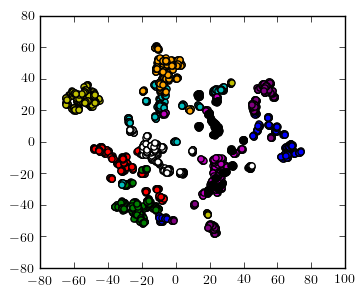
\includegraphics[height=3.1cm]{gls_modelnet10_codes_}
        \subcaption{\bf \DVAE t-SNE}
        \label{fig:results-latent-space-a1}
    \end{subfigure}
    \hspace*{-12px}
    \begin{subfigure}[t]{0.49\linewidth}
        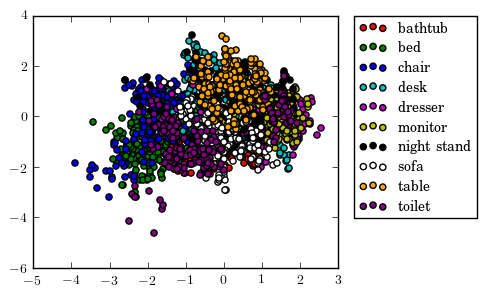
\includegraphics[height=3cm]{gls_modelnet10_codes2}
        \subcaption{\bf \DVAE Projection}
        \label{fig:results-latent-space-a2}
    \end{subfigure}
    \\
    \hspace*{-22px}
    \begin{subfigure}[t]{0.49\linewidth}
        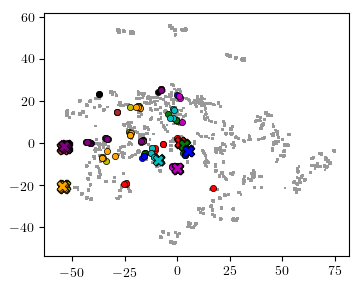
\includegraphics[height=3cm]{gls_clean_codes_outputs_}
        \subcaption{\bf \AML t-SNE}
        \label{fig:results-latent-space-b1}
    \end{subfigure}
    \hspace*{-12px}
    \begin{subfigure}[t]{0.49\linewidth}
        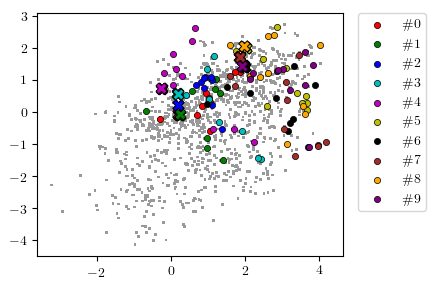
\includegraphics[height=3cm]{gls_clean_codes2_outputs}
        \subcaption{\bf \AML Projection}
        \label{fig:results-latent-space-b2}
    \end{subfigure}
    \vspace*{-\figskipcaption px}
    \caption{{\bf Learned Latent Spaces.} In (\subref{fig:results-latent-space-a1}) and (\subref{fig:results-latent-space-a2}), we show a t-SNE \citep{Maaten2008JMLR} visualization and a two-dimensional projection of the \DVAE latent space on ModelNet10. The plots illustrate that the \DVAE is able to separate the ten object categories. In (\subref{fig:results-latent-space-b1}) and (\subref{fig:results-latent-space-b2}), we show a t-SNE visualization and a projection of the latent space corresponding to our learned \AML model on \clean. We randomly picked $10$ ground truth shapes,  ``x'', and the corresponding observations ($10$ per shape), points (gray pixels indicate remaining shapes/observations). The plots illustrate that \AML is able to associate observations with the corresponding ground truth shapes under weak supervision.}
    \label{fig:results-latent-space}
    \vspace*{-\figskipbelow px}
\end{figure}
\begin{table*}[t]
    \vspace*{-\figskipabove px}
    \centering
    {\scriptsize
        \begin{tabularx}{1\textwidth}{|@{  }l@{  }|@{  }X@{  }|@{  }c@{  }c@{  }c@{  }c@{  }|@{  }c@{  }c@{  }c@{  }c@{  }|@{  }c@{  }|}
            \hline
             \multicolumn{1}{|@{  }c@{  }|@{  }}{Supervision} & \multicolumn{1}{@{  }c@{  }|@{  }}{Method} & \multicolumn{4}{@{  }c@{  }|@{  }}{\clean} & \multicolumn{4}{@{  }c@{  }|@{  }}{\noisy} & \multicolumn{1}{c|}{KITTI}\\
             \multicolumn{1}{|@{  }c@{  }|@{  }}{in \%} && \Abs {\tiny $\downarrow$} & \IoU {\tiny $\uparrow$} & \Acc [vx] {\tiny $\downarrow$} & \Compl [vx] {\tiny $\downarrow$} & \Abs {\tiny $\downarrow$} & \IoU {\tiny $\uparrow$} & \Acc [vx] {\tiny $\downarrow$} & \Compl [vx] {\tiny $\downarrow$} & \Compl [m] {\tiny $\downarrow$} \\
            \hline\hline
            \multicolumn{11}{|c|}{Low Resolution: $24 \times 54 \times 24$ voxels; * independent of resolution}\\
            \hline\hline
            {\color{darkgray}(shape prior)} & {\leavevmode\color{darkgray}\DVAE} & {\color{darkgray}0.019} & {\color{darkgray}0.885} & {\color{darkgray}0.283} & {\color{darkgray}0.527} & \multicolumn{5}{@{  }c@{  }|}{{\color{darkgray}(same shape prior as on \clean)}}\\
            \hline\hline
            \multirow{2}{*}{$\hphantom{<}100$} & \cite{Dai2017CVPRa} (\Dai) & {\bf\color{rred} 0.021} & {\bf\color{rred} 0.872} & {\bf\color{rred} 0.321} & {\bf\color{rred} 0.564} & {\bf\color{rred} 0.027} & {\bf\color{rred} 0.836} & {\bf\color{rred} 0.391} & {\bf\color{rred} 0.633} & 0.128\\
            &\Sup & 0.026 & 0.841 & 0.409 & 0.607 & 0.028 & 0.833 & 0.407 & 0.637 & {\bf\color{rred} 0.091}\\
            \hline
            \multirow{10}{*}{$<7.7$} &\BL & 0.067 & 0.596 & 0.999 & 1.335 & 0.064 & 0.609 & 0.941 & 1.29 & \color{darkgray}--\\
            &\M & 0.052 & 0.697 & 0.79 & 0.938 & 0.052 & 0.696 & 0.79 & 0.938 & \color{darkgray}--\\
            &\ML & 0.04 & 0.756 & 0.637 & 0.8 & 0.041 & 0.755 & 0.625 & 0.829 & \color{darkgray}(too slow)\\
            & *\cite{Gupta2015CVPR} (\ICP) & \multicolumn{2}{@{  }c@{  }}{\color{darkgray}(mesh only)} & 0.534 & {\bf\color{rgreen} 0.503} & \multicolumn{2}{@{  }c@{  }}{\color{darkgray}(mesh only)} & 7.551 & 6.372 & \color{darkgray}(too slow)\\
            & *\cite{Engelmann2016GCPR} (\Engelmann) & \multicolumn{2}{@{  }c@{  }}{\color{darkgray}(mesh only)} & 1.235 & 1.237 & \multicolumn{2}{@{  }c@{  }}{\color{darkgray}(mesh only)} & 1.974 & 1.312 & 0.13\\ % 0.545016
            &\dAML & {\bf\color{rgreen} 0.034} & {\bf\color{rgreen} 0.784} & {\bf\color{rgreen} 0.532} & 0.741 & {\bf\color{rgreen} 0.036} & {\bf\color{rgreen} 0.772} & {\bf\color{rgreen} 0.557} & {\bf\color{rgreen} 0.76} & \color{darkgray}(see \AML)\\
            &\AML & {\bf\color{rgreen} 0.034} & 0.779 & 0.549 & 0.753 & {\bf\color{rgreen} 0.036} & 0.771 & 0.57 & 0.761 & {\bf\color{rgreen} 0.12}\\
            \hline\hline
            \multicolumn{11}{|c|}{Low Resolution: $24 \times 54 \times 24$ voxels; Multiple, $k > 1$ Fused Views}\\
            \hline\hline
            \multirow{2}{*}{$\hphantom{<}100$} & \cite{Dai2017CVPRa} (\Dai), $k = 5$ & \bf\color{rred}0.012 & \bf\color{rred}0.924 & \bf\color{rred}0.214 & \bf\color{rred}0.436 & \bf\color{rred}0.018 & \bf\color{rred}0.887 & \bf\color{rred}0.278 & \bf\color{rred}0.491 &\multirow{2}{*}{\color{darkgray}n/a}\\
            &\Sup, $k = 5$ & 0.022 & 0.866 & 0.336 & 0.566 & 0.024 & 0.86 & 0.331 & 0.573 &\\
            \hline
            $<16$ & \AML, $k = 2$ & 0.032 & 0.794 & 0.489 & 0.695 & 0.034 & 0.79 & 0.52 & 0.725 & \multirow{3}{*}{\color{darkgray}n/a}\\
            $<24$ & \AML, $k = 3$ & {\bf\color{rgreen} 0.031} & {\bf\color{rgreen} 0.809} & {\bf\color{rgreen} 0.471} & {\bf\color{rgreen} 0.667} & {\bf\color{rgreen} 0.031} & {\bf\color{rgreen} 0.81} & {\bf\color{rgreen} 0.493} & {\bf\color{rgreen} 0.67} &\\
            $<40$ & \AML, $k = 5$ & {\bf\color{rgreen} 0.031} & 0.804 & 0.502 & 0.686 & 0.035 & 0.799 & 0.523 & 0.7 &\\
            \hline\hline
            \multicolumn{11}{|c|}{Medium Resolution: $32 \times 72 \times 32$ voxels}\\
            \hline\hline
            {\color{darkgray}(shape prior)} & {\leavevmode\color{darkgray}\DVAE} & {\color{darkgray}0.019} & {\color{darkgray}0.877} & {\color{darkgray}0.24} & {\color{darkgray}0.47} & \multicolumn{5}{@{  }c@{  }|}{{\color{darkgray}(same shape prior as on \clean)}}\\
            \hline\hline 
            \multirow{2}{*}{$\hphantom{<}100$} & \cite{Dai2017CVPRa} (\Dai) & {\bf\color{rred} 0.02} & {\bf\color{rred} 0.869} & {\bf\color{rred} 0.399} & {\bf\color{rred} 0.674} & {\bf\color{rred} 0.026} & {\bf\color{rred} 0.83} & {\bf\color{rred} 0.51} & {\bf\color{rred} 0.767} & {\bf\color{rred} 0.074}\\
            &\Sup & 0.027 & 0.834 & 0.498 & 0.789 & 0.029 & 0.815 & 0.571 & 0.843 & 0.09\\
            \hline
            $\leq6.1$ & \AML & {\bf\color{rgreen} 0.031} & {\bf\color{rgreen} 0.788} & {\bf\color{rgreen} 0.415} & {\bf\color{rgreen} 0.584} & {\bf\color{rgreen} 0.036} & {\bf\color{rgreen} 0.766} & {\bf\color{rgreen} 0.721} & {\bf\color{rgreen} 0.953} & {\bf\color{rgreen} 0.083}\\
            \hline\hline
            \multicolumn{11}{|c|}{High Resolution: $48 \times 108 \times 48$ voxels}\\
            \hline\hline
            {\color{darkgray}(shape prior)} & {\leavevmode\color{darkgray}\DVAE} & {\color{darkgray}0.018} & \color{darkgray}0.87 & {\color{darkgray}0.272} & {\color{darkgray}0.434} & \multicolumn{5}{@{  }c@{  }|}{{\color{darkgray}(same shape prior as on \clean)}}\\
            \hline\hline
            \multirow{2}{*}{$\hphantom{<}100$} & \Dai & {\bf\color{rred} 0.017} & {\bf\color{rred} 0.88} & {\bf\color{rred} 0.517} & {\bf\color{rred} 0.827} & 0.054 & 0.664 & 1.559 & 2.067 & {\bf\color{rred} 0.066}\\
            &\Sup & 0.023 & 0.843 & 0.677 & 1.032 & {\bf\color{rred} 0.052} & {\bf\color{rred} 0.674} & {\bf\color{rred} 1.52} & {\bf\color{rred} 1.981} & 0.091\\
            \hline
            $<3.5$ & \AML & {\bf\color{rgreen} 0.028} & {\bf\color{rgreen} 0.796} & {\bf\color{rgreen} 0.433} & {\bf\color{rgreen} 0.579} & {\bf\color{rgreen} 0.045} & {\bf\color{rgreen} 0.659} & {\bf\color{rgreen} 1.4} & {\bf\color{rgreen} 1.957} & {\bf\color{rgreen} 0.078}\\
            \hline
        \end{tabularx}
    }
    \vspace*{-\figskipcaption px}
    \caption{{\bf Quantitative Results on ShapeNet and KITTI.} We consider Hamming distance (\Abs) and intersection over union (\IoU) for occupancy grids as well as accuracy (\Acc) and completeness (\Compl) for meshes on \clean, \noisy and KITTI. For \Abs, \Acc and \Compl, lower is better; for \IoU, higher is better. The unit of \Acc and \Compl is voxels (voxel length at $24 \ntimes 54 \ntimes 48$ voxels) or meters. Note that the \DVAE shape prior (in {\color{darkgray}gray}) is only reported as reference (\ie, bound on (d)\AML). We indicate the level of supervision in percentage, relative to the corresponding resolution and mark the best results under full supervision in {\color{rred}\bf red} and under weak supervision in {\color{rgreen}\bf green}.}
    \label{tab:results-shapenet}
    \vspace*{-\figskipbelow px}
\end{table*}

Inspired by the work by \cite{Gupta2015CVPR} we also consider a shape retrieval and fitting baseline. Specifically, we perform iterative closest point (\ICP) \citep{Besl1992PAMI} fitting on all training shapes and subsequently select the best-fitting one. To this end, we uniformly sample $1\text{Mio}$ points on the training shapes, and perform point-to-point \ICP\footnote{\url{http://www.cvlibs.net/software/libicp/}.} for a maximum of $100$ iterations using $\left[\begin{matrix}R & t\end{matrix}\right] = \left[\begin{matrix}I_3 & 0\end{matrix}\right]$ as initialization. On the training set, we verified that this approach is always able to retrieve the perfect shape.

Finally, we consider a simple \ML baseline iteratively minimizing \eqnref{eq:ml} using stochastic gradient descent (SGD). This baseline is similar to the work by Engelmann \etal, however, like ours it is bound to the voxel grid. Per example, we allow a maximum of $5000$ iterations, starting with latent code $z = 0$, learning rate $0.05$ and momentum $0.5$ (decayed every $50$ iterations at rate $0.85$ and $1.0$ until $10^{-5}$ and $0.9$ have been reached).

\boldparagraph{Learning-Based Approaches}
%
Learning-based approaches usually employ an encoder-decoder architecture to directly learn a mapping from observations $x_n$ to ground truth shapes $y_n^*$ in a fully supervised setting \citep{Wang2017ICCV,Varley2017IROS,Yang2018ARXIVb,Yang2017ARXIV,Dai2017CVPRa}. While existing architectures differ slightly, they usually rely on a U-net architecture \citep{Ronneberger2015MICCAI,Cicek2016ARXIV}. In this paper, we use the approach of \cite{Dai2017CVPRa}\footnote{
    We use \url{https://github.com/angeladai/cnncomplete}. On ModelNet we added one convolutional stage in the en- and decoder for larger resolutions; on ShapeNet and KITTI, we needed to adapt the convolutional strides to fit the corresponding resolutions.
} -- referred to as \Dai\xspace --
as a representative baseline for this class of approaches. In addition, we consider a custom learning-based baseline which uses the architecture of our \DVAE shape prior, \cf \figref{fig:architectures}. In contrast to \citep{Dai2017CVPRa}, this baseline is also limited by the low-dimensional ($Q = 10$) bottleneck as it does not use skip connections.